\section{Методика использования программного средства}
\label{sec:manual}

В данном разделе приведены основные сведения по работе с программным средством. 
Приложение доступно в AppStore и Android Market.
Рассмотрим основные функции, предоставляемые приложением пользователям.

При запуске приложение появляется экран с регистрацией/авторизацией (рисунок~\ref{fig:manual:login}).
Если пользователь забыл пароль, то он может его изменить, нажав на
соответствующую кнопку.

\begin{figure}[H]
\centering
	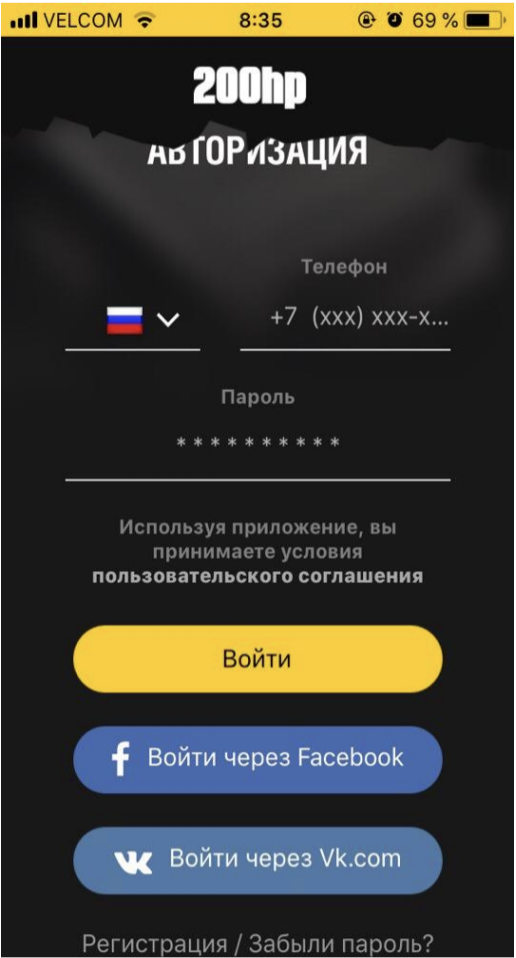
\includegraphics[scale=0.6]{manual/login-screen.png}
	\caption{Экран авторизации}
	\label{fig:manual:login}
\end{figure}

Пользователь может зарегистрироваться с помощью номера телефона и
пароля, либо с помощью учётных данных от социальных сетей «Вконтакте»
или Facebook (рисунок ~\ref{fig:manual:auth}).

\begin{figure}[H]
  \centering
    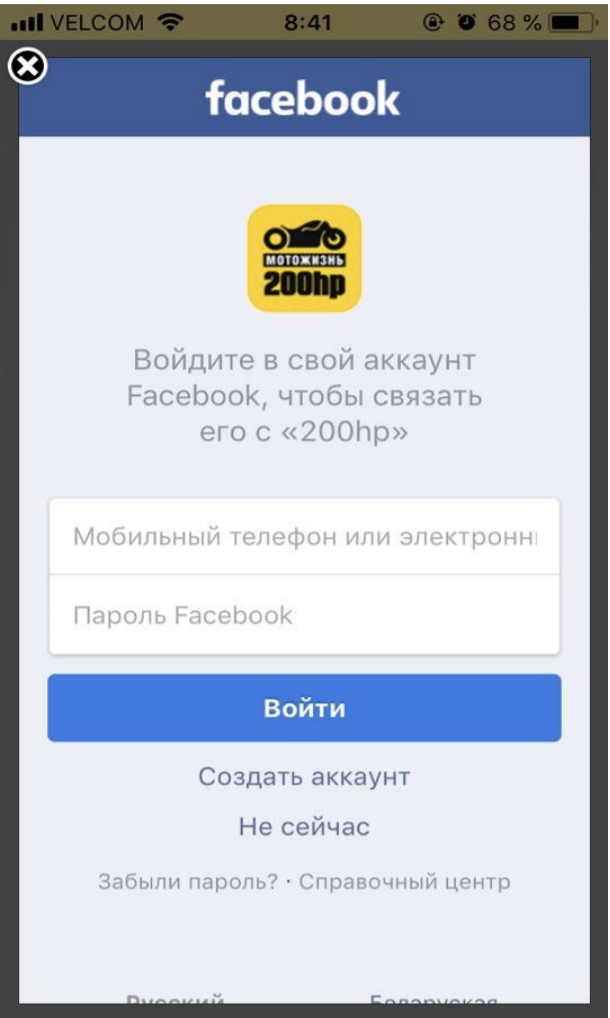
\includegraphics[scale=0.5]{manual/facebook-screen.png}
    \caption{Авторизация/вход через Facebook}
    \label{fig:manual:auth}
  \end{figure}

Профиль пользователя представлен на рисунке~\ref{fig:manual:profile}.

\begin{figure}[H]
  \centering
    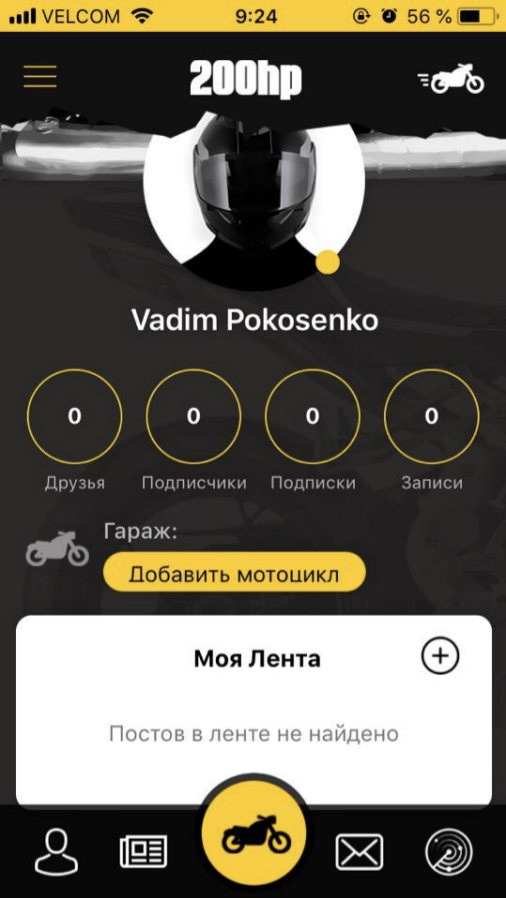
\includegraphics[scale=0.6]{manual/profile-screen.png}
    \caption{Профиль пользователя}
    \label{fig:manual:profile}
  \end{figure}

После нажатия кнопки «Применить» появляется страница, где
пользователь может увидеть фотографию (рисунок~\ref{fig:manual:creatingPost}), добавить к ней
комментарии, которые могут включать хештеги для облегчения поиска постов
по соответствующей тематике.

\begin{figure}[H]
    \centering
      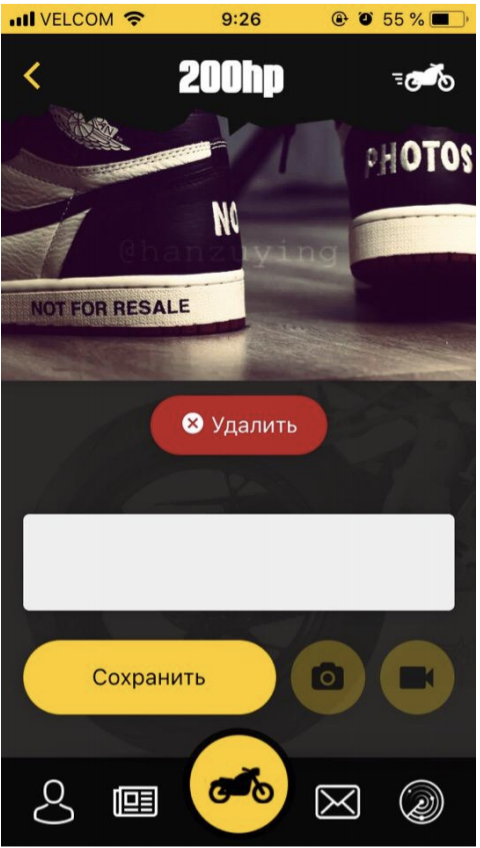
\includegraphics[scale=0.6]{manual/creating-post.png}
      \caption{Создание поста}
      \label{fig:manual:creatingPost}
\end{figure}

После нажатия кнопки «Сохранить» пост появляется в ленте (рисунок~\ref{fig:manual:uploadedPost}). Друзья смогут увидеть вашу запись, написать комментарий к ней и
лайкнуть.

\begin{figure}[H]
  \centering
    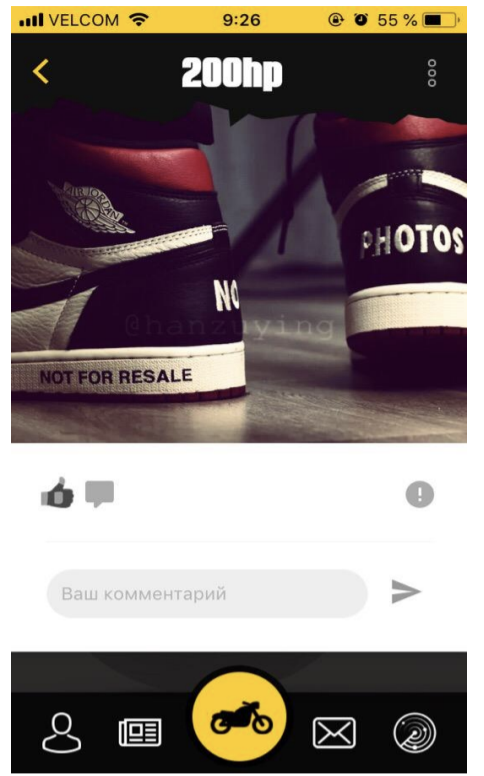
\includegraphics[scale=0.6]{manual/uploaded-post.png}
    \caption{Лента пользователя с добавленной записью}
    \label{fig:manual:uploadedPost}
\end{figure}

Процесс загрузки фото и видео точно такой же, как и при добавлении
постов в ленту пользователя. После нажатия кнопки сохранить появляется
обновлённый гараж с записью о мотоцикле (рисунок~\ref{fig:manual:bike}).

\begin{figure}[H]
  \centering
    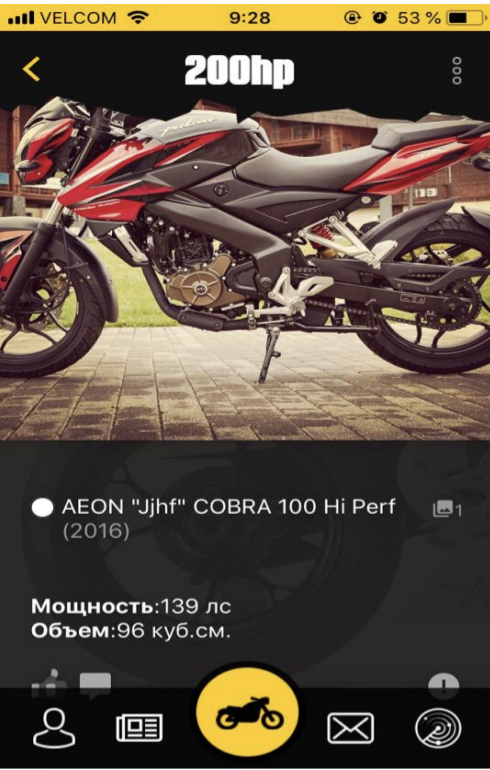
\includegraphics[scale=0.6]{manual/bike.png}
    \caption{Гараж}
    \label{fig:manual:bike}
\end{figure}

Пользователь может принять запрос, просмотреть профиль
пользователя либо игнорировать его, в этом случае он останется в
подписчиках. При нажатии пункта добавить в друзья обновляется счётчик
друзей в профиле, и вы можете вести переписку (рисунок~\ref{fig:manual:dialog}).

\begin{figure}[H]
  \centering
    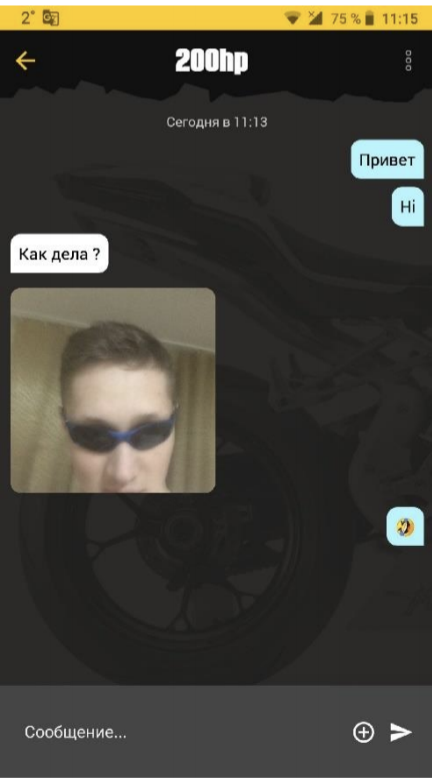
\includegraphics[scale=0.6]{manual/dialog.png}
    \caption{Переписка}
    \label{fig:manual:dialog}
\end{figure}

Карта местности с метками друзей, кнопкой получения текущего
расположения, и установки меток представлена на рисунке\ref{fig:manual:map}.

\begin{figure}[H]
  \centering
    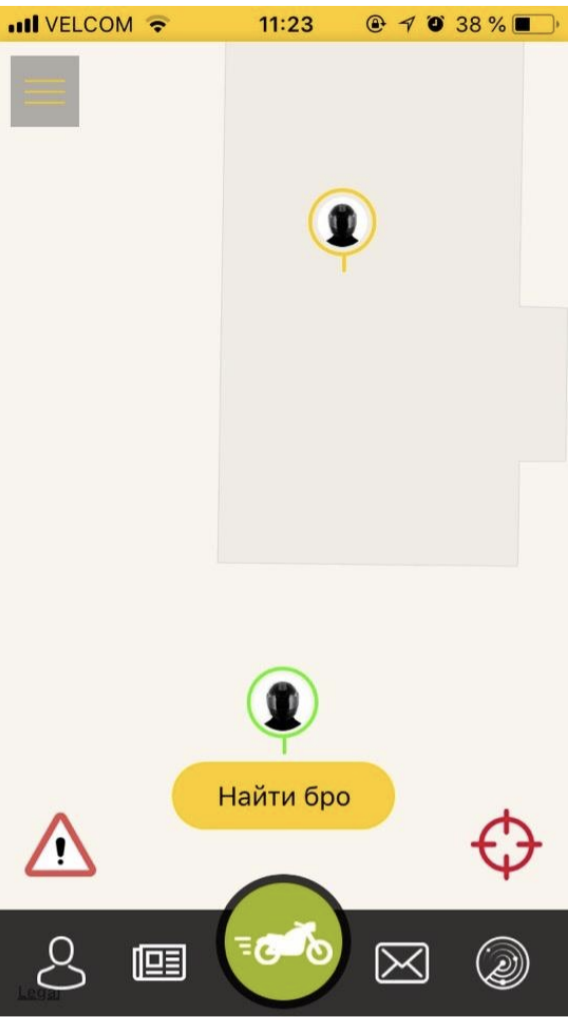
\includegraphics[scale=0.6]{manual/map.png}
    \caption{Карта}
    \label{fig:manual:map}
\end{figure}


Таким образом, в данном разделе приведены примеры использования некоторых их основных возможностей разработанного программного средства.
